\chapter{Simulation results for generating arbitrary signals}
Output measurement with harmonic balance simulator in agilent design system in time domain for different signal bandwidths (e.g. \SI{125}{\MHz}, \num{500e6} Hz, 1GHz). The transistor models used in agilents design system was generated at IAF. Which exact model? In addition to this, the simulation is done with ideal condition. no conductor losses, nor bond inductance are considered.\\
Different signals are simulated using this digital-to-analog converter. These signals were generated with a resolution of 3-bit and a oversampling ratio of four. The generated signal bandwidth is depending on the control frequency (sampling frequency).
% This belongs to the fundamentals and concept
%$OSR = 2^{r} = 4$. Hence the factor $r = 2$ which is used in the diagrams provided by the french mathematics. 
\\ The digital control sequence, the riemanncode, is based on the weights of the slopes and is generated by hand. Fig. \ref{fig:SineWaveCodeGeneration} show the optical generation of the riemanncode.

\begin{enumerate}
	\item Vout simulation: three-bit resolution, osr = 4, BW limits: DC to 6GHz$\rightarrow$ could not be processed, manufactured while the period of the thesis. 
	\begin{itemize}
		\item sine ;produce every signal out of sine wave (fourier transformation)
		\item half sine ;only as an example
		\item triangular ;only as an example
	\end{itemize}
	\item Vout simulation: two-bit resolution, osr = 4, keep it small and simple, frequency higher, demonstrator, assembly, less complex
	\begin{itemize}
		\item sine
		\item half sine ;only as an example
		\item triangular ;only as an example
	\end{itemize}
	\item S-parameter - load impedance		
	\item Switch voltage - necessary?
	\item Max Gain with output amp - to tune the quiescent point, get the right impdenace
	\item stability 
	\item energy consumption
\end{enumerate}
Explain Bandwidth limitations. The lower bound is determined by the sampling time (inverse of the sampling frequency;) and the smallest current achieved with the dimensioned transistors. The smallest achievable current times the smallest sampling time (highest sampling frequency) determine the smallest absolute slope achievable. \\ \textbf{Is every signal possible to create? The signal bandwidth ranges from DC to 6 GHz but what is the amplitude range? Is there a limitation regarding the amplitude?}
\\
The smallest current is determined by the dimension of the transistor, which drives into saturation. The smallest saturated current is determined by the push-pull transistor geometry, here: 532 mA.\\Voltage across capacitor is determined by:

\begin{itemize}
	\item Harmonic Balance simulation is used to neglect the transient time (steady-state)
	\item S-parameter simulation is done for the matching, determining impedance
	\item Stability simulation is done to check whether or not oscillation occurs
	\item energy consumption is determined by the HB simulation; more or less
\end{itemize}

%% Important: appearance(format) all the same, same frequency, sam oversamplingratio, same resolution, et cetera
% create this figure/picture
%\begin{figure}[ht]
%	\centering
%  \includegraphics[width=1\textwidth, draft]{DAC_generated_sine_wave.png}
%	\caption{Digital to analog converted signal representing a sine wave using ads simulation}
%	\label{DAC_generated_sine_wave}
%\end{figure}

\section{Time signal simulation with three bit resolution DAC and optimized component dimensions}
The dimension of the used components is based on chapter "Dimension of the used components". The output voltage of this circuit is simulated in time domain.
A digitally controlled charge pump with eight different slopes is created, called Riemann Pump. To show that this pump is able to convert a digital signal into an analog one an example code is generated. As a MATLAB algorithm do not exists, which computes the Riemann Code, it is done by hand.

\subsection{sine wave}
This example code represents a signal which approach to be a sine wave. The sequence of slope is the following: \textit{+7 +3 -3 -7 -7 -3 +3 +7}.
A theoretical created sine wave is compared to the synthesized sine wave with the riemann pump simulation. As seen in Figure \ref{fig:SineCompare} the synthesized signal is very close to the theoretical optimal. The deviation is very small hence the signal to noise ratio is very low. As in equation \ref{eq:SNR_RiemannPumpConversion} stated the snr is calculated.


 \begin{figure}[htb!]
   \centering
   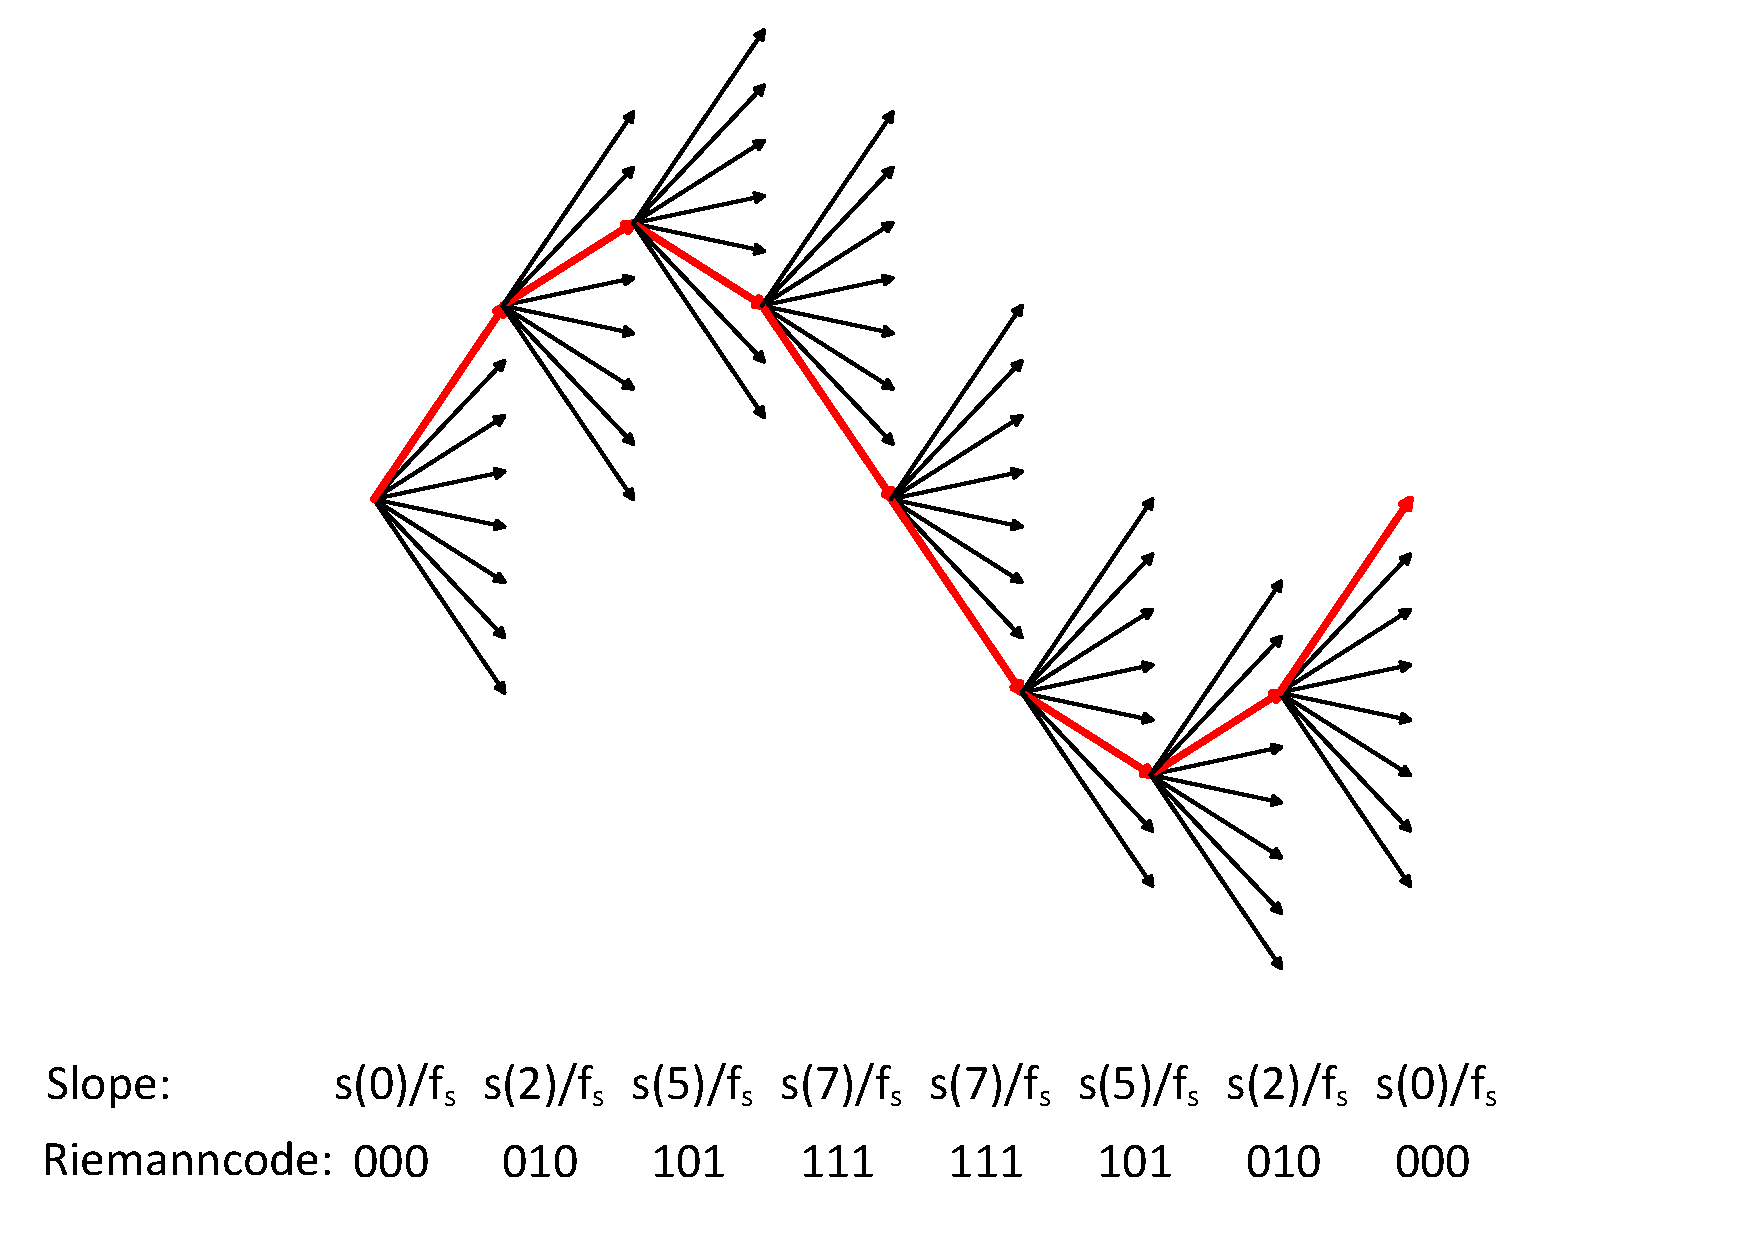
\includegraphics[width=1\textwidth]{SineWaveGenerationByHand.pdf}
   \caption{Riemanncode generation for a sine wave by hand}
   \label{fig:SineWaveCodeGeneration}
\end{figure}
 
With this riemanncode mentioned in fig \ref{fig:SineWaveCodeGeneration} signals with different signal frequency are simulated. Based on the sampling frequency and the oversampling ratio of four (OSR=4) the following signals were generated.

\begin{figure}[htb!]
   \centering
   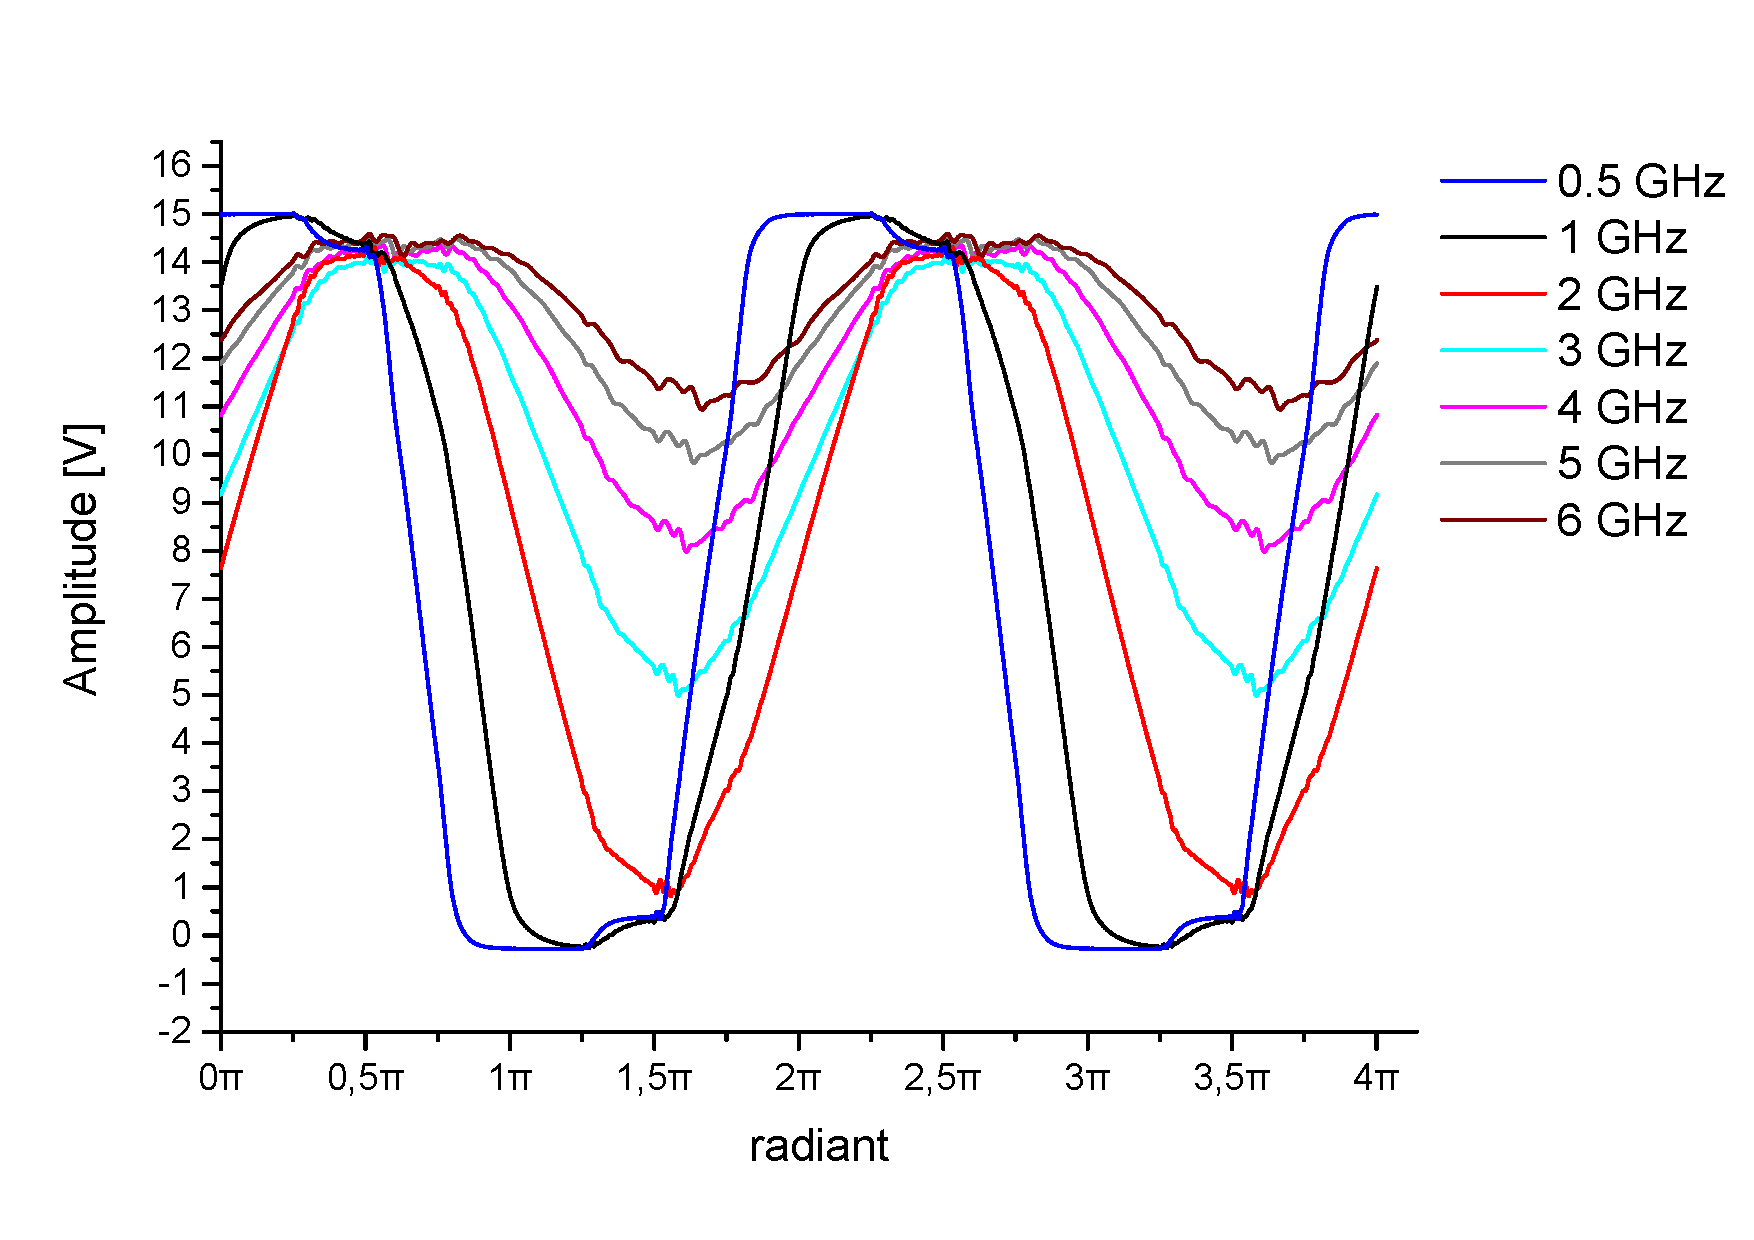
\includegraphics[width=0.75\textwidth]{Vout_sine_7signals_inOne_3bit_osr4.pdf}
   \caption{Signals based on the riemann code in fig \ref{fig:SineWaveCodeGeneration}}
   \label{fig:SineWavesGeneration}
\end{figure}
 
No MATLAB algorithm exists which calculates the optimal code, minimizing the error, for controlling the digital to analog converter. Based on the components dimension and the generated Riemanncode in Fig. \ref{fig:SineWaveCodeGeneration} with the corresponding sampling frequency the following theoretical sine wave can be generated

\begin{figure}[htb!]
   \centering
   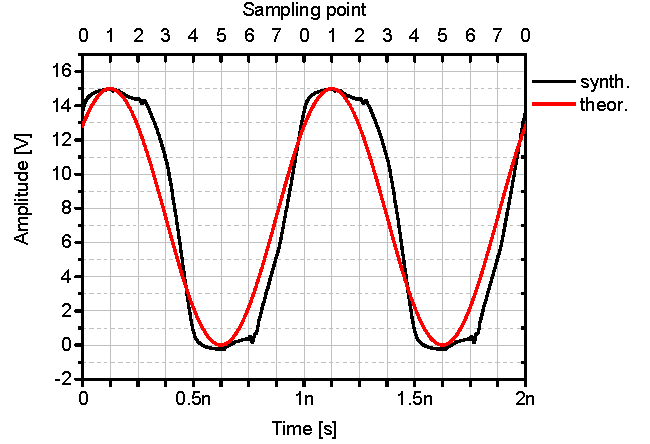
\includegraphics[width=0.75\textwidth]{Vout_SynthVsTheo.pdf}
   \caption{Synthesized sine wave with the theoretical sine wave}
   \label{fig:SineWaveSynthVsTheoretical}
\end{figure}
In fig. \ref{fig:SineWaveSynthVsTheoretical} the following signal is generated:
\begin{equation}
v(t)= \widehat{v} \cdot sin( 2  \pi  f \cdot  t + \phi)
\end{equation}
with this parameter: $\widehat{v} = \SI{7.5}{\volt}$, $f = \SI{1}{\giga \hertz}$, $\phi = \pi / 4$


\begin{figure}[htb!]
	\centering
  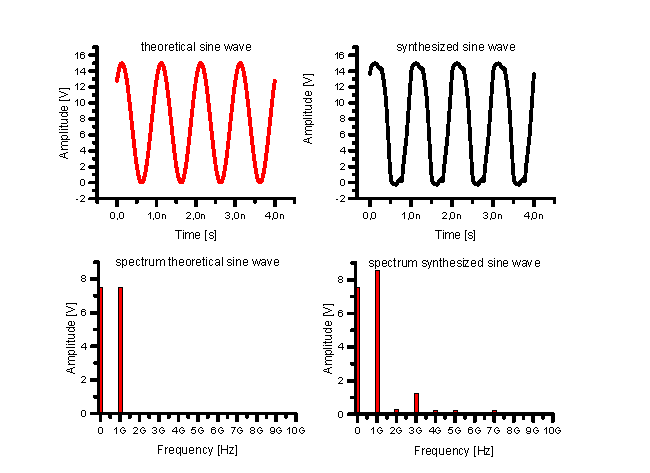
\includegraphics[width=1\textwidth]{SineCompare.pdf}
	\caption{Comparison between a theoretical and a synthesized sine wave with their spectrum}
	\label{fig:SineCompare}
\end{figure}


Figure \ref{fig:1GHz sine} shows a sine wave with a frequency of 1 GHz synthesized with the DAC. The control frequency is eight times the signal bandwidth.
\begin{figure}[htb!]
   \centering
   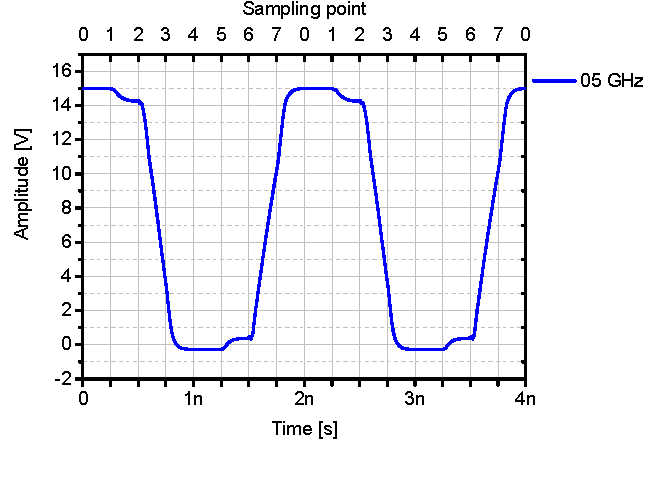
\includegraphics[width=0.75\textwidth]{Vout_sine_SigBW_05GHz_3bit_long.pdf}
   \caption{amplitude of a synthesized sine wave with signal frequency of 500 MHz, $f_{sampling} =$ \SI{4}{\GHz} in the time domain}
   \label{fig:05GHz sine}
\end{figure}
\begin{figure}[htb!]
   \centering
   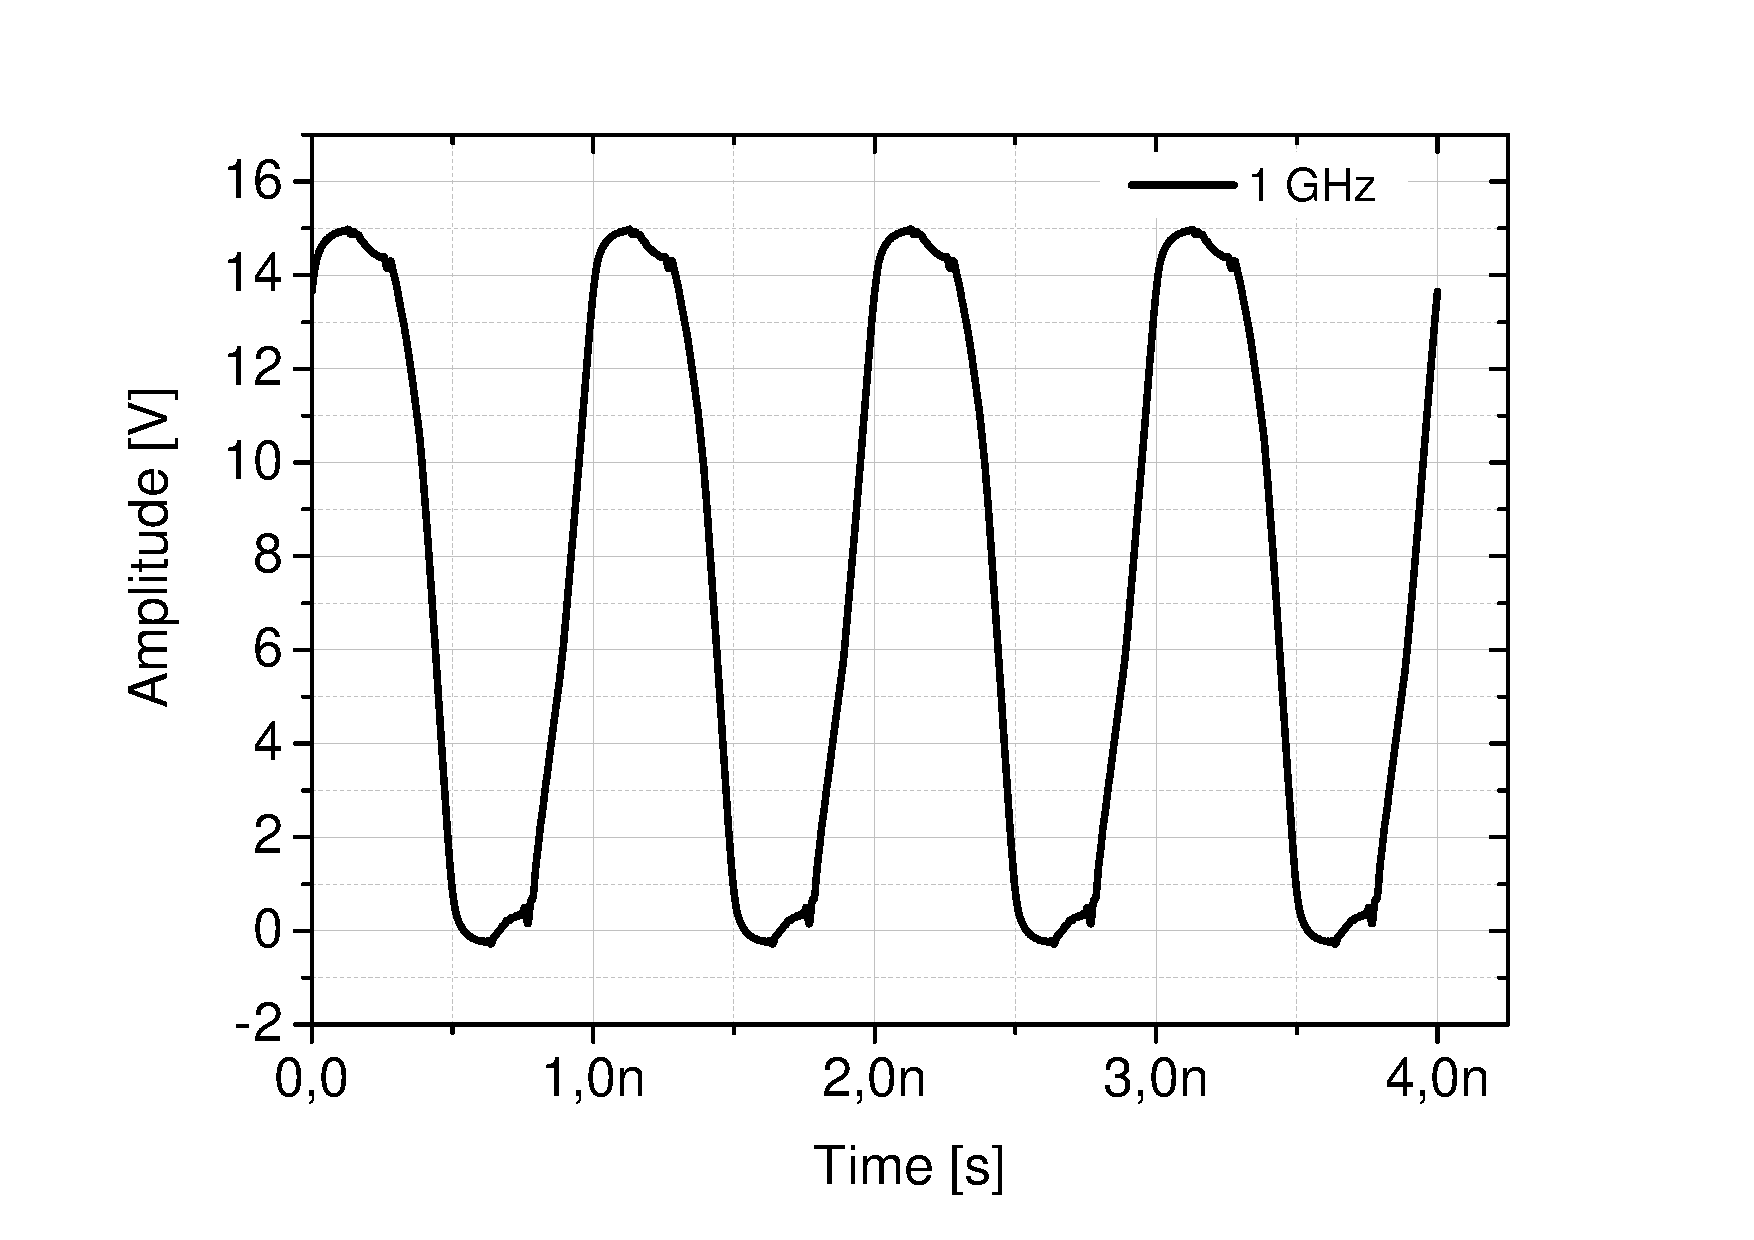
\includegraphics[width=0.75\textwidth]{Vout_sine_SigBW_1GHz_3bit_long.pdf}
   \caption{amplitude of a synthesized sine wave with signal frequency of 1 GHz, $f_{sampling} =$ \SI{8}{\GHz} in the time domain}
   \label{fig:1GHz sine}
\end{figure}
\begin{figure}[htb!]
   \centering
   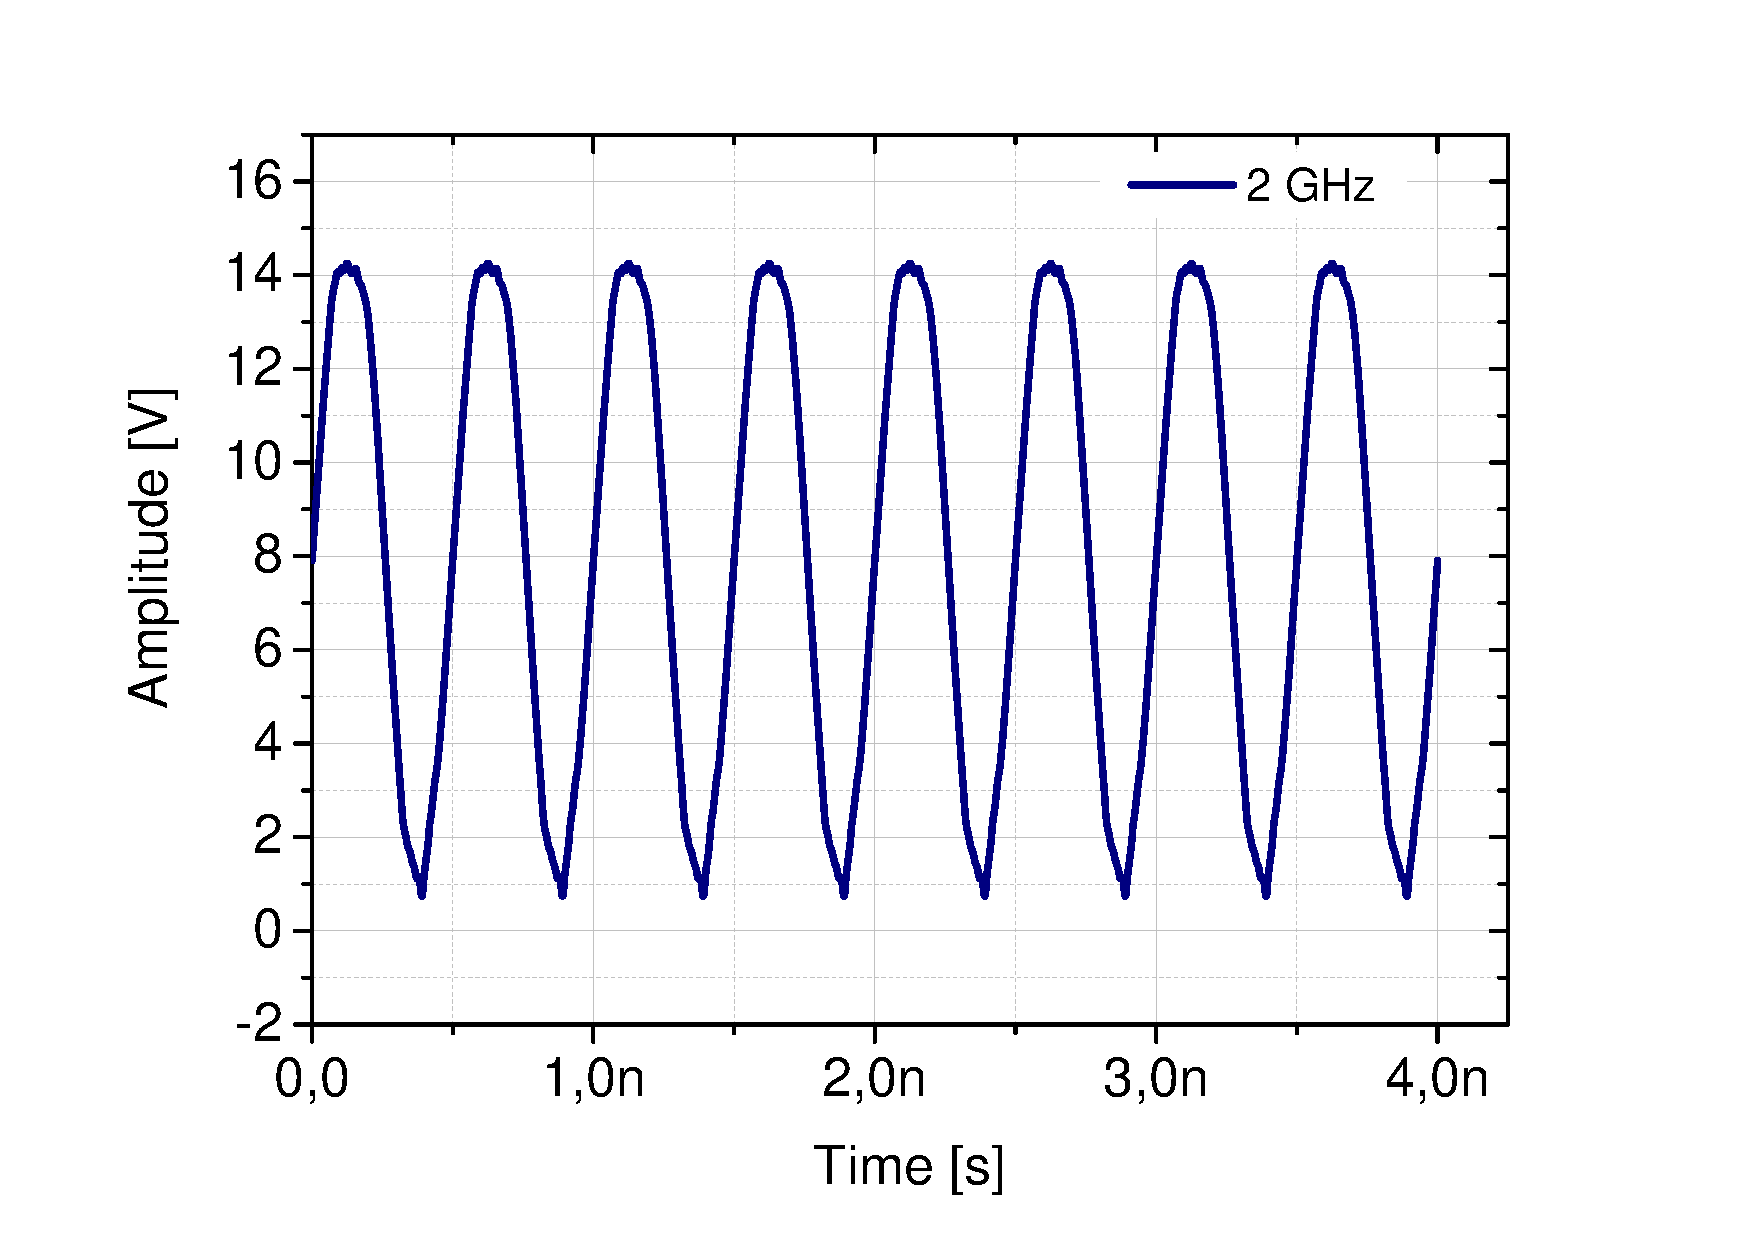
\includegraphics[width=0.75\textwidth]{Vout_sine_SigBW_2GHz_3bit_long.pdf}
   \caption{amplitude of a synthesized sine wave with signal frequency of 2 GHz, $f_{sampling} =$ \SI{16}{\GHz} in the time domain}
   \label{fig:2GHz sine}
\end{figure}




This signal is generated with the riemann code. This riemann code was obtained by hand with optical estimation with the slopes obtained from the table.
\subsection{half sine}
Based on the same optical approximation of the signal in Fig. \ref{fig:SineWaveCodeGeneration} the riemanncode for the half sine is generated. The Riemanncode for the half sine is: 000 010 101 111 000 010 101 111
\subsection{triangular}
This is a triangular wave.
%
%\begin{figure}
%\centering
%\begin{minipage}{.5\linewidth}
%  \centering
%  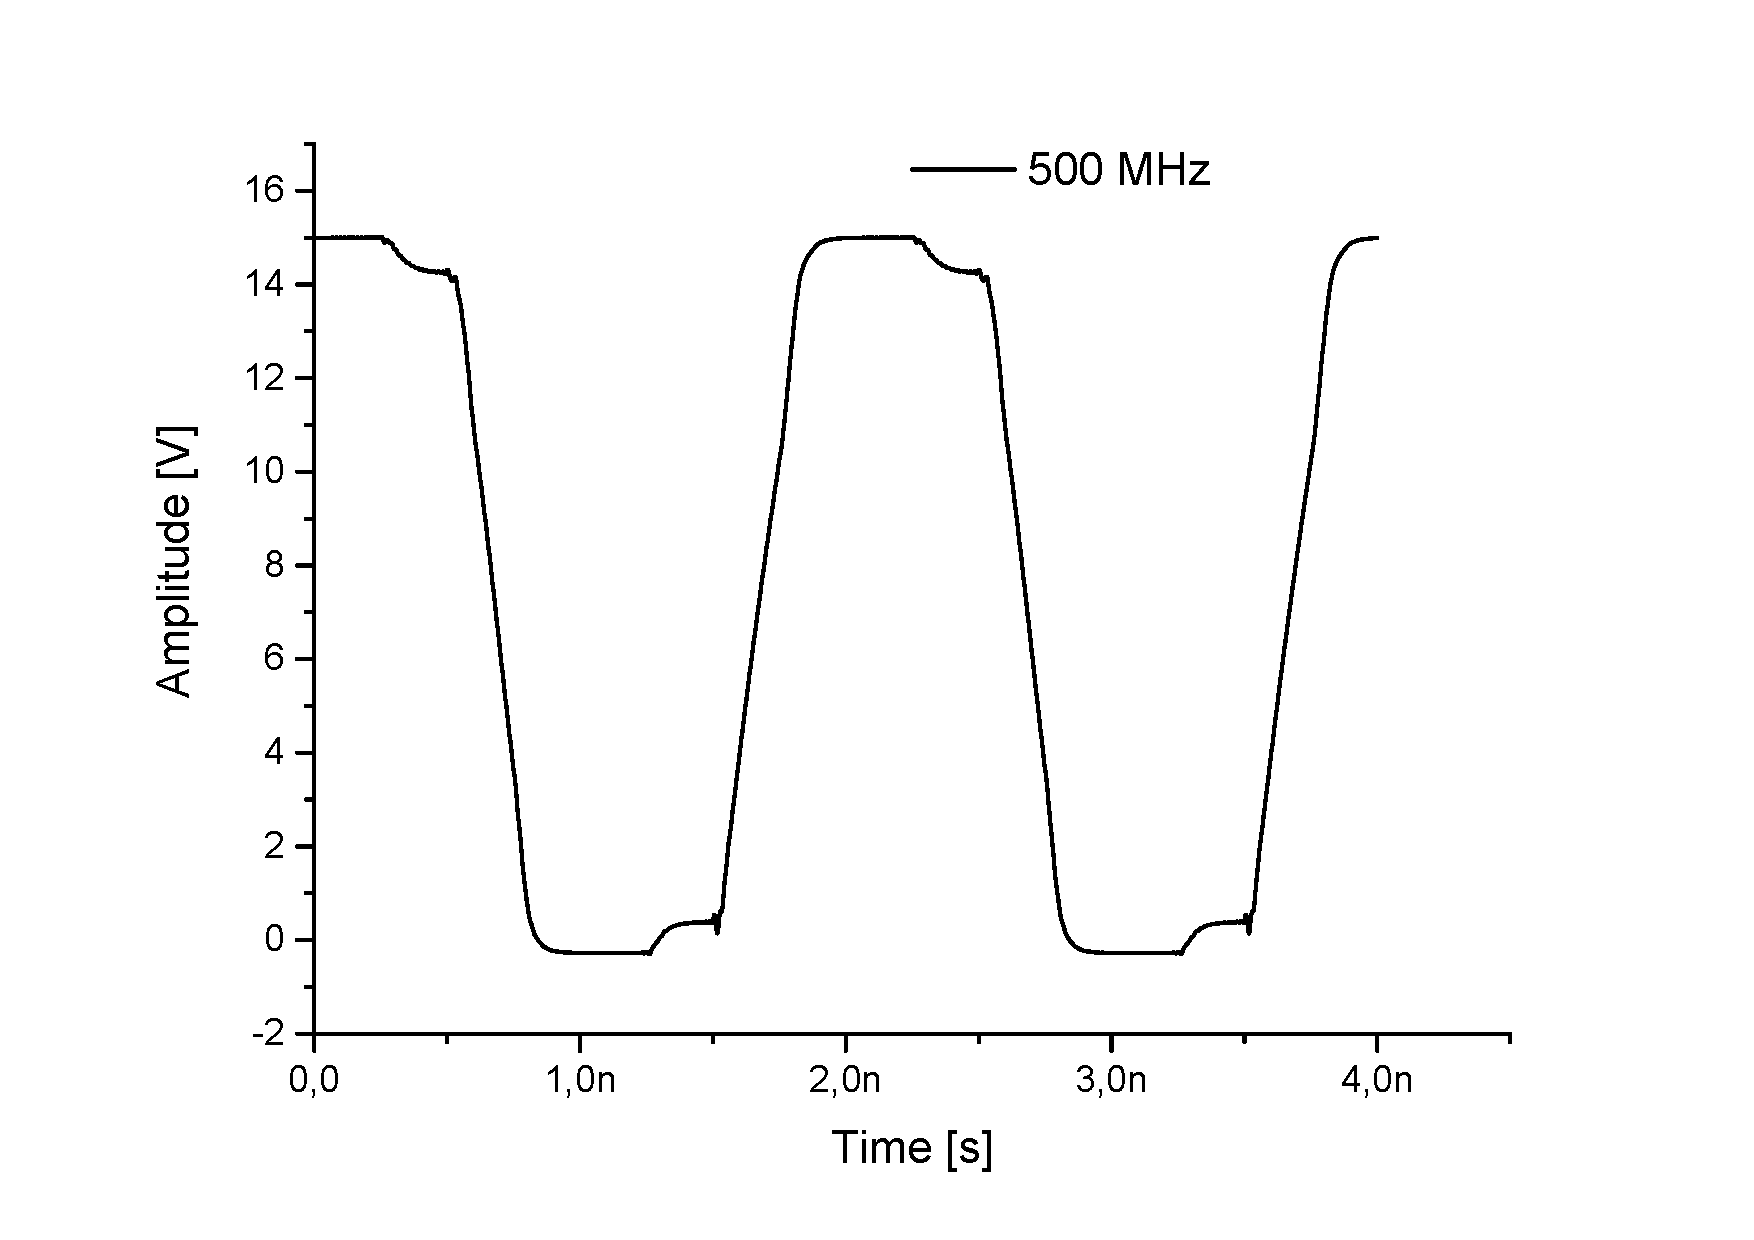
\includegraphics[width=1\linewidth]{Vout_sine_SigBW_05GHz_3bit.pdf}
%  %\caption{500 MHZ signal}
%  \label{fig:test1}
%\end{minipage}%
%\begin{minipage}{.5\linewidth}
%  \centering
%  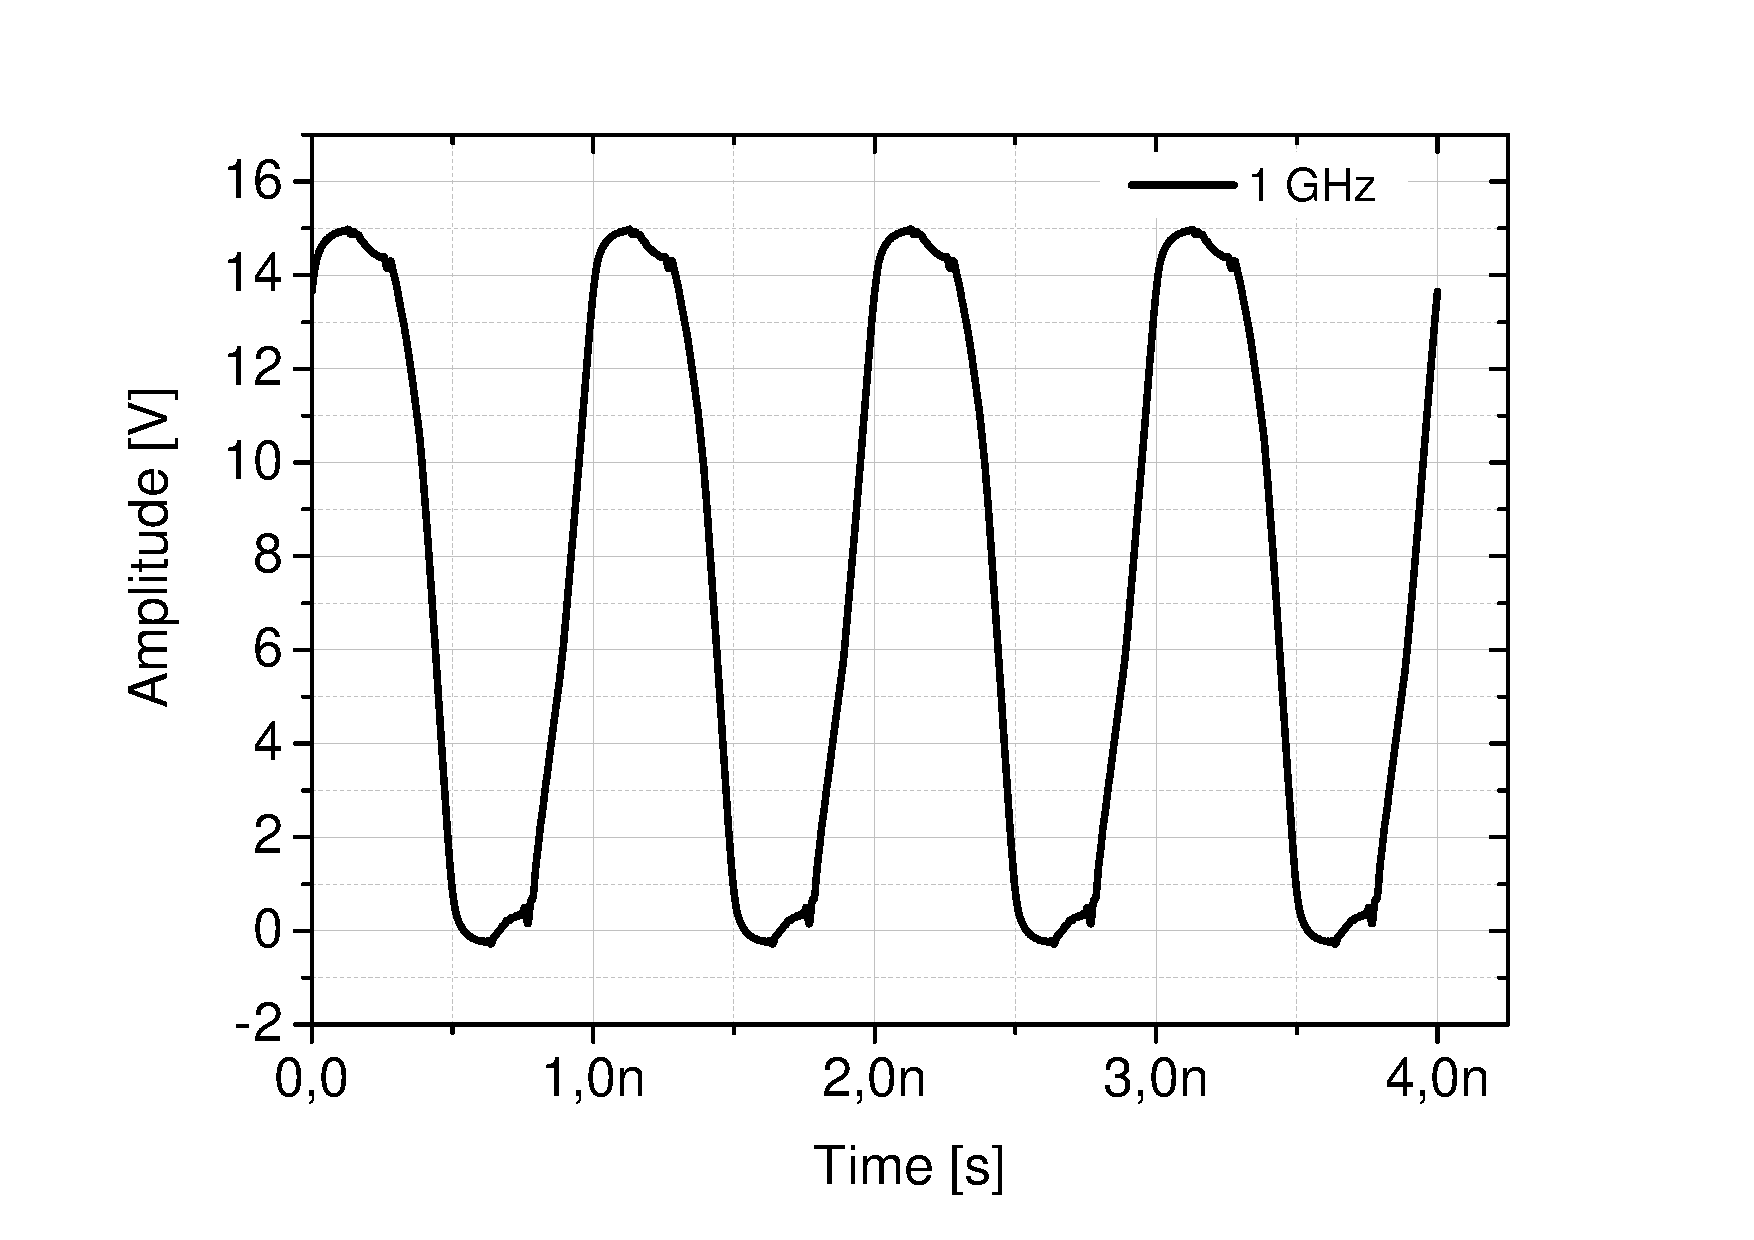
\includegraphics[width=1\linewidth]{Vout_sine_SigBW_1GHz_3bit_long.pdf}
%  %\caption{2 GHz}
%  \label{fig:test2}
%\end{minipage}
%%\end{figure}
%%
%%
%%\begin{figure}
%\centering
%\begin{minipage}{.5\linewidth}
%  \centering
%  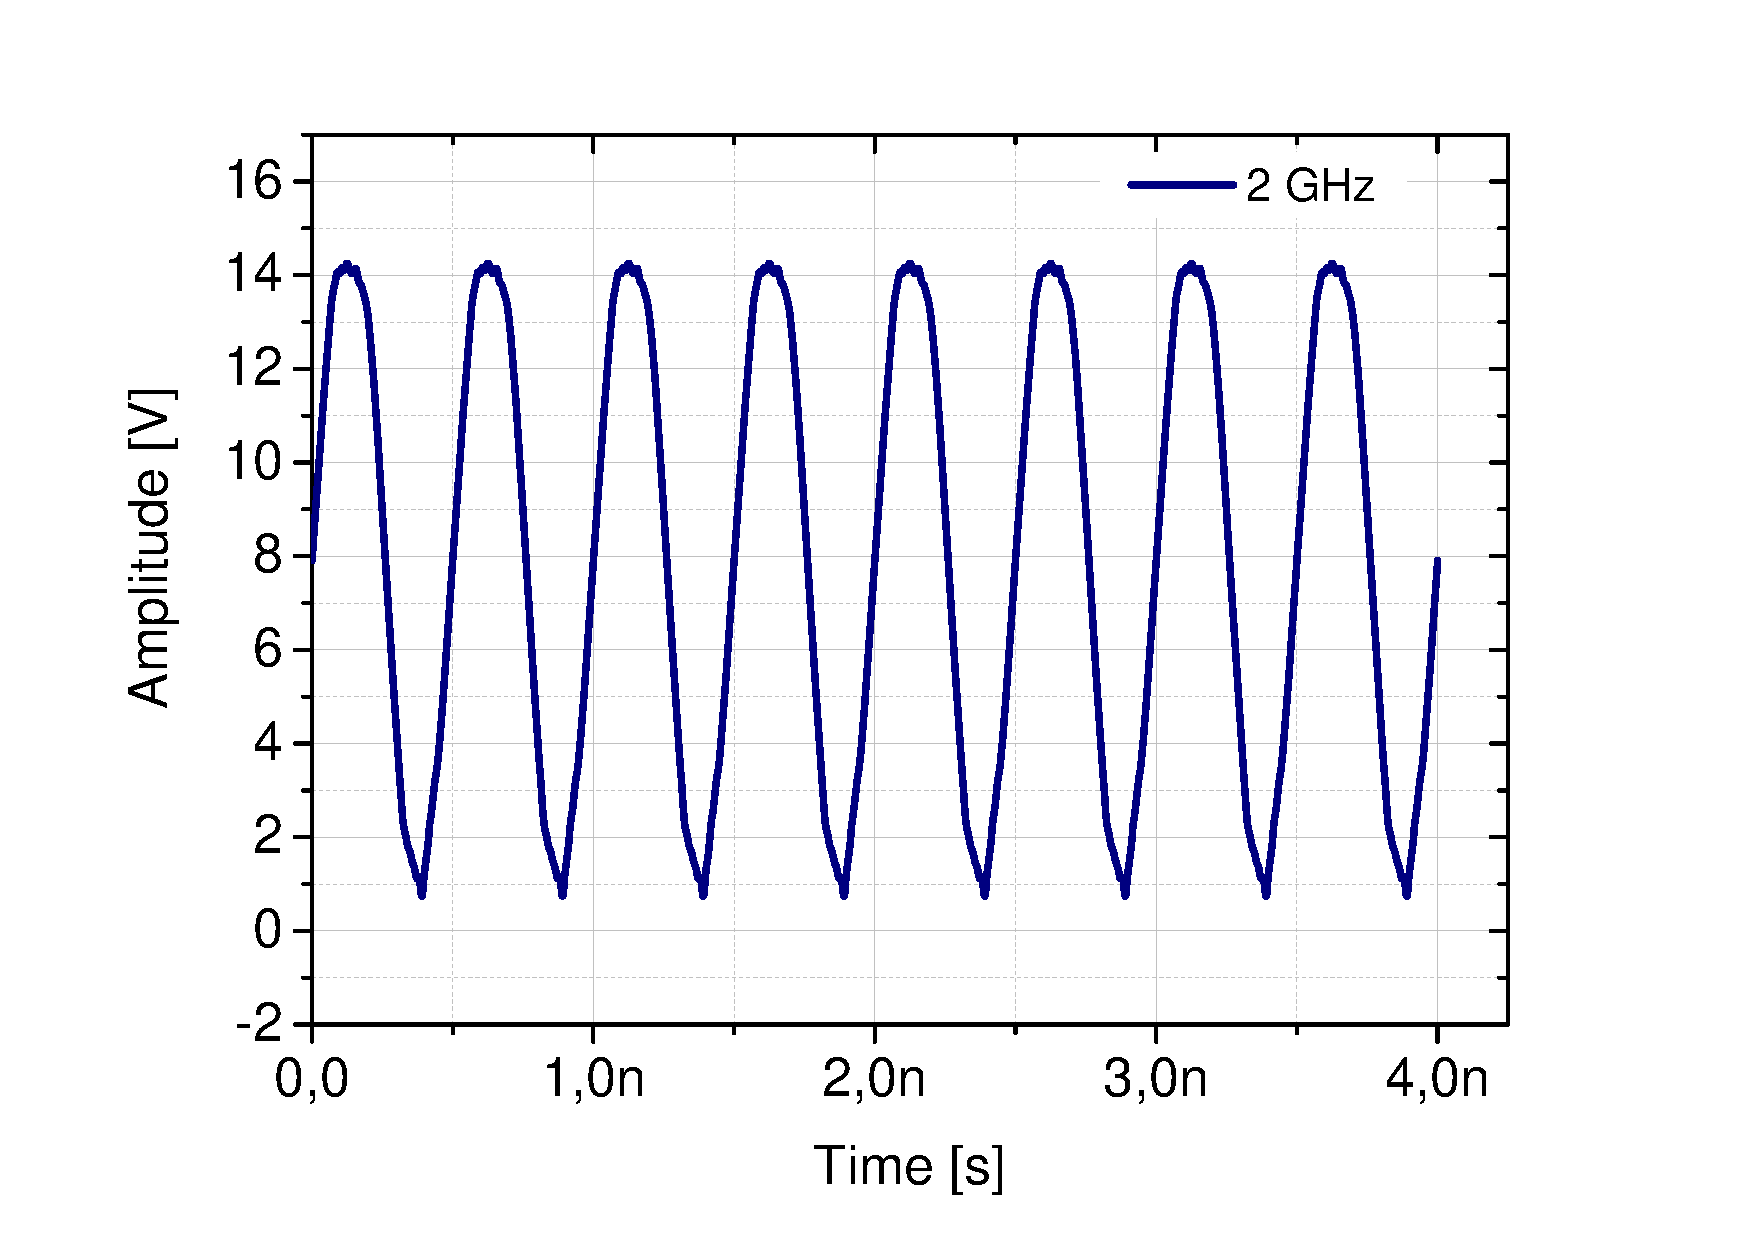
\includegraphics[width=1\linewidth]{Vout_sine_SigBW_2GHz_3bit_long.pdf}
% % \caption{1GHZ signal}
%  \label{fig:test3}
%\end{minipage}%
%\begin{minipage}{.5\linewidth}
%  \centering
%  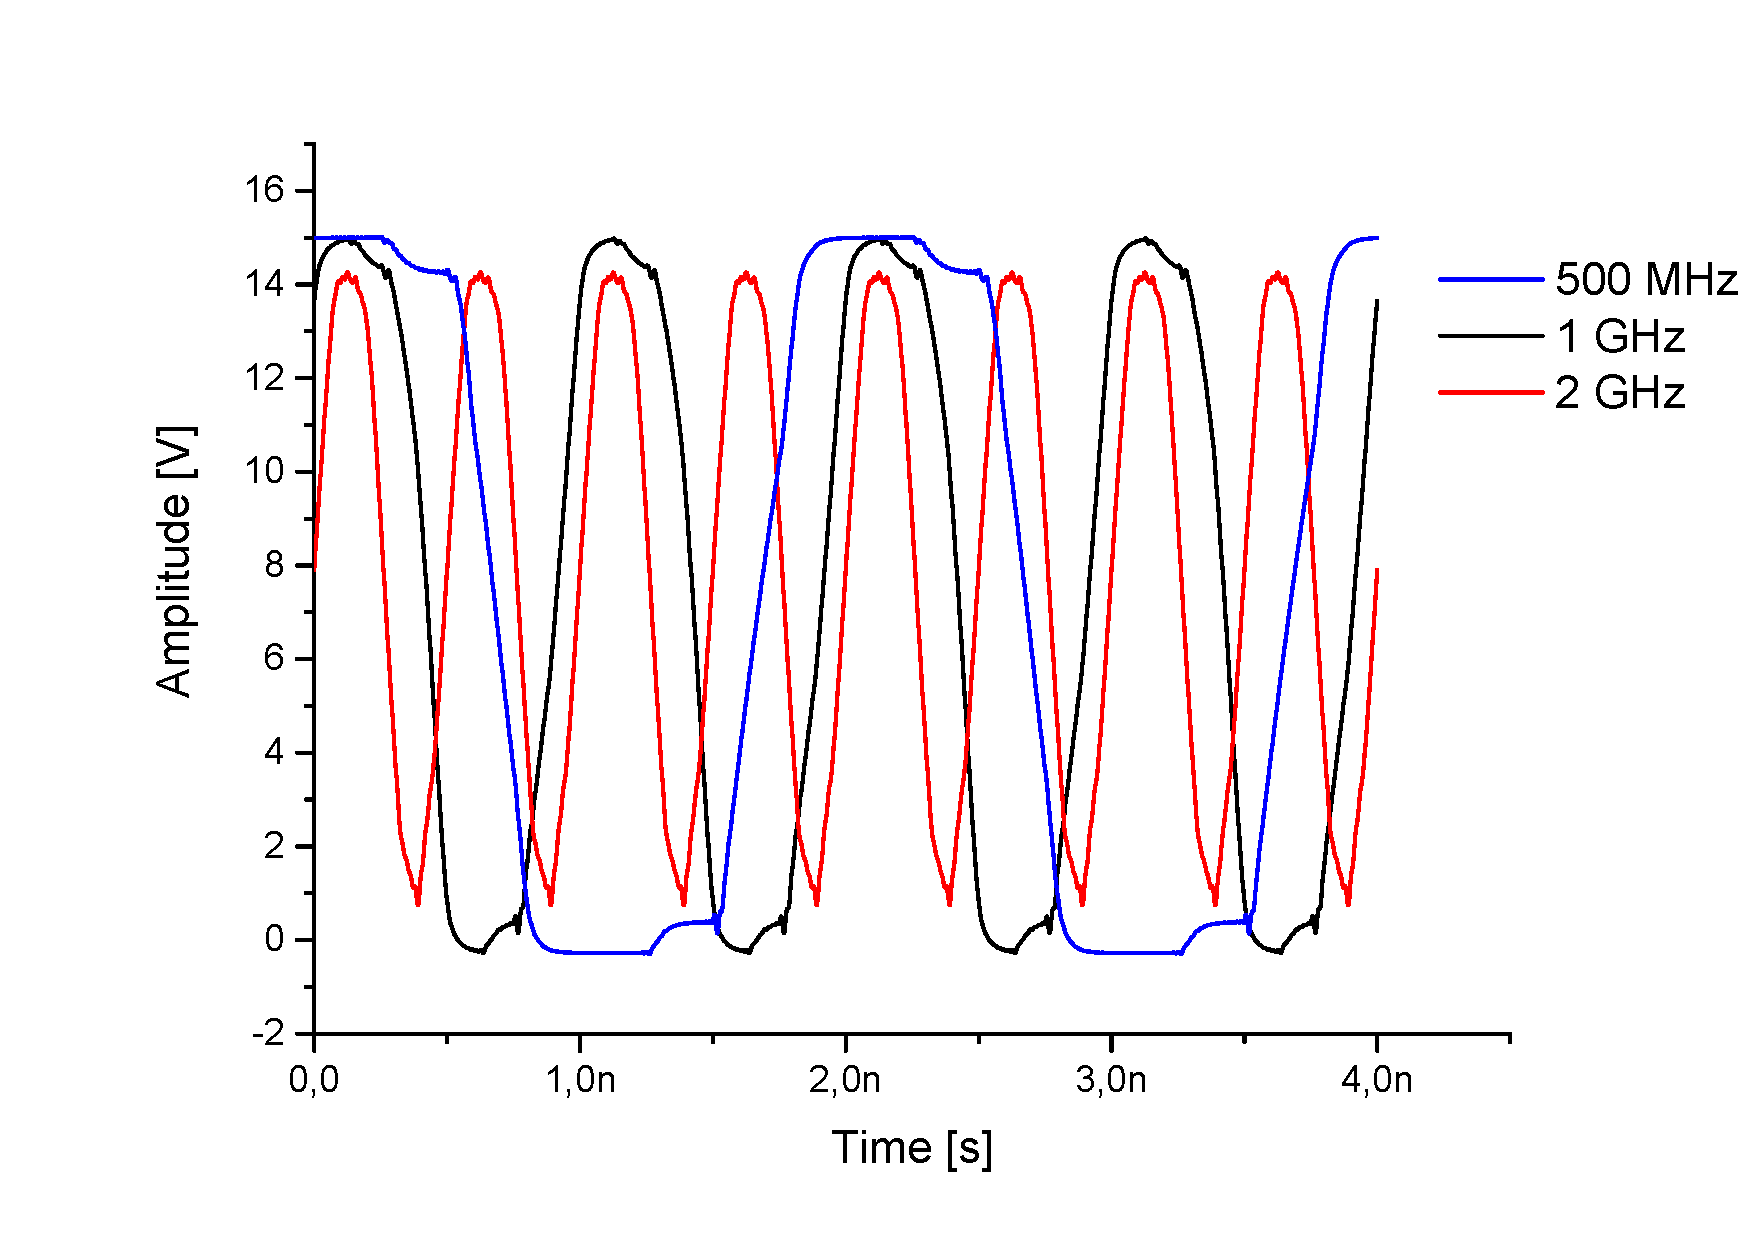
\includegraphics[width=1\linewidth]{Vout_sine_SigBW_ALL_3bit.pdf}
%%  \caption{2 GHz}
%  \label{fig:test4}
%\end{minipage}
%\end{figure}


\section{Time signal simulation with two bit resolution dac and component dimension like demonstrator}
This two bit resolution simulation is done to compare the demonstrators measurements with the simulation. The three bit resolution DAC was too complex to realize in a first approach on a hybrid substrate
\subsection{differences of three signals which can be compared to measurements}
Here to present the two bit resolution sine wave, half sine wave and triangular

\section{Stability analysis}
A stability analysis is done within the ADS tool. This should state that the corresponding circuit do not oscillate at specific frequencies or frequency ranges.

\section{Energy consumption analysis}
The energy consumption is analysed with the circuit created by me in ADS. For the chips used for the demonstrator refer to the work of Stephan Maroldt who states, that the power consumption is:  divided into static and dynamic ones. The switching losses are greater than the static ones.
